\subsection{Propuesta}
\label{propuesta}

Por lo analizado en capítulos anteriores, se propone una arquitectura más desacoplada a la planteada con el Integrador, permitiendo de esta manera minimizar el costo del mantenimiento, desarrollo y simplificando su despliegue en entornos de producción. Una solución basada en estándares que permita integrar sistemas heterogéneos, aceptando el hecho de que la mayoría de los sistemas legados que se encuentran en producción, se mantendrán y logrando de esta manera, que la infraestructura subyacente facilite la incorporación de cambios que puedan surgir como necesidades del {\cespi} y la {\unlp}.

El modelo de servicios facilita el acceso y consumo de la información a través de la red. Dado que los servicios son independientes y autónomos, pueden combinarse tantas veces como sea necesario de manera sencilla, generando nuevas aplicaciones que respondan a las necesidades en constante evolución de nuestra casa de estudios. Esta posibilidad de agregar y combinar servicios para resolver situaciones presentes y futuras, convierten en una opción altamente beneficiosa el uso de esta estrategia, con el fin de crear servicios y aplicaciones complejas con independencia de las tecnologías subyacentes\cite{microsoft2006}.

El resultado final es una nube, con un conjunto de servicios y una creciente flota de aplicaciones dependientes de éstos, que se adapta fácilmente a los cambios.

A continuación profundizaremos la aplicación concreta de los conceptos vistos hasta aquí, explicando nuestra propuesta a través de los puntos mencionados en el objetivo al comienzo del presente trabajo.

\subsubsection{Redundancia y escalabilidad}
\label{propuesta:escalabilidad}

Cuando hablamos de escalabilidad, podemos basarnos en el modelo llamado \eng{scale cube}\cite{website:akfpartners-scale-cube} presentado visualmente en la \autoref{fig:scale-cube}. Este modelo clasifica las distintas formas de escalar las aplicaciones en 3 sentidos, tomando como analogía las 3 dimensiones de un cubo:

\begin{itemize}
  \item \textbf{Escalar sobre el eje \textit{X}:} (\eng{X-axis scaling}, en inglés) Técnica comúnmente utilizada para incrementar la disponibilidad de las aplicaciones. Consiste en el uso de instancias replicadas de la aplicación (idénticas a la original), ubicadas detrás de un balanceador de carga que reparte el trabajo entre ellas.
  \item \textbf{Escalar sobre el eje \textit{Y}:} (\eng{Y-axis scaling}, en inglés) Ésta es una técnica que se encuentra en auge con el \textit{momentum} que están teniendo los microservicios. Se basa en la descomposición funcional de la aplicación en un conjunto de servicios colaborativos, donde cada uno implementa una parte específica de las funciones. En este caso, la disponibilidad se incrementa al separar en componentes más pequeñas la unidad funcional mayor que es la aplicación, dividiendo el trabajo independientemente entre ellas.
  \item \textbf{Escalar sobre el eje \textit{Z}:} (\eng{Z-axis scaling}, en inglés) En este enfoque se toma como base la replicación de instancias presente en \eng{X-axis scaling} y a esto se agrega una capa superior de abstracción que separa el conjunto de datos que cada instancia o instancias atenderá, acorde a algún criterio lógico como puede ser el cliente que realice la petición (privilegiando unos clientes sobre otros).
\end{itemize}

\begin{figure}
  
\includegraphics[width=\linewidth]{src/images/04-capitulo-4/scale-cube.png}
  \caption{El modelo de escalabilidad \eng{scale cube}}
  \label{fig:scale-cube}
\end{figure}

Como vimos en el Capítulo I, el diseño de la arquitectura del Integrador presenta falencias que no permiten implementar redundancia ni escalar de manera eficiente, ya que para poder hacerlo, encontramos al menos dos inconvenientes: para lograr redundancia, sería necesario replicar su instancia virtual y al mismo tiempo implementar alguna solución que redirija las peticiones a cualquiera de sus réplicas.  Además, debido a su diseño arquitectónico, sería necesario replicar cada \gls{acro:api}, pero como se mencionó anteriormente, éstas se encuentran fuertemente acopladas a sus aplicaciones, lo que fuerza a replicar no sólo la \gls{acro:api}, sino también la aplicación que genera los datos.

Debido a esto, planteamos una nueva arquitectura de la nube de servicios de la {\unlp} que debe ser replicable y escalable. Para lograrlo, cada \gls{acro:api} correrá en una instancia virtual independiente, de manera tal que la misma pueda ser replicada tantas veces como sea necesario (\eng{X-axis scaling}). La capa de abstracción de estas instancias replicadas será un balanceador de carga, implementado con \nameref{soa:tecnologias:nginx}, que servirá tanto para balancear la carga, como de \eng{failover}, dando continuidad a los servicios en caso de que alguna de las instancias replicadas falle.

La característica fundamental de un balanceador de carga es ser capaz de distribuir las peticiones entrantes a un grupo de servidores (\eng{backends}) de acuerdo a un algoritmo de decisión y ponderación llamado \eng{scheduler}. Este algoritmo seleccionará qué backend podría atender un requerimiento entrante, existiendo algunos simples (hacerlo de manera aleatoria o siguiendo un criterio ordenado por turnos como \eng{Round Robin}) y otros más sofisticados (que consideran otros factores como por ejemplo la carga de cada backend, su tiempo de respuesta promedio, el número de conexiones activas, la ubicación geográfica, etc.). En su funcionamiento básico el balanceador de carga redirige las peticiones a alguno de los backends, el cual luego contesta al balanceador, para que finalmente sea el balanceador el que entregue la respuesta al cliente sin que este último sepa de la existencia de esta compleja arquitectura. Esta estructura transparente al cliente evita accesos directos entre éste y los servidores que actúan como backend.

Como se mencionó anteriormente, el balanceador puede también ser usado como \eng{failover}, permitiendo que la falla de uno o más backends no afecten la disponibilidad del servicio. Los backends son monitoreados continuamente por el balanceador, cuando uno de éstos falla, el balanceador deja de enviar tráfico al backend caído. Una vez que el backend vuelve a estar online, el balanceador detecta esta situación y comienza a enviarle tráfico nuevamente.

Para disminuir la cantidad de accesos que llegan a las instancias replicadas de los servicios, delante del balanceador se implementará una caché compartida utilizando \nameref{soa:tecnologias:varnish}, la cual evitará los accesos innecesarios al mantener una copia en memoria de las respuestas que alguna de las instancias replicadas de la {\cloud} haya generado, obteniendo mejores tiempos de respuesta así como tolerancia a fallos y reducción de carga en estas últimas.

A modo de ejemplo, podemos pensar en una aplicación (\textit{cliente A}) que accede al servicio \url{/academic_units}. La petición es atendida por la API de referencia, donde el servicio devuelve todas la Unidades Académicas activas. Si más tarde otra aplicación (\textit{cliente B}), consulta la \gls{acro:api} por las Unidades Académicas, accediendo también al servicio \url{/academic_units} de la misma API, terminará obteniendo el mismo listado de Unidades Académicas. Como se puede apreciar, tenemos dos accesos a la API de referencia con idénticas respuestas, ambas procesadas por completo por alguno de los backends. Esta situación puede evitarse con la inclusión de una cache compartida delante del balanceador de carga, logrando mejorar los tiempos de respuesta ya que la API recibirá únicamente un acceso, debiendo acceder y procesar los datos una única vez, ya que el resto de las peticiones serán obtenidas desde la cache compartida.


\subsubsection{Desacoplamiento}

Como se mencionó en la \autoref{esb:introduccion} (ESB), uno de los 9 principios de diseño de \gls{acro:soa} es el bajo acoplamiento (\eng{loose coupling}), y quizás la forma más común de implementarlo es mediante un \gls{acro:esb}, el cual se encargará de proveer interoperabilidad entre las diferentes plataformas.  En nuestra arquitectura proponemos utilizar \nameref{soa:tecnologias:tyk} como ESB delante del \nameref{soa:tecnologias:varnish} para agregar mecanismos de autenticación, \eng{rate limiting}, monitoreo y un único punto de acceso a toda la {\cloud}, el cual estará restringido a las direcciones IP de las aplicaciones cliente. La inclusión del ESB evita la necesidad de desarrollar en las \glspl{acro:api} funcionalidad extra, que este mismo provee.

Al mismo tiempo, en pos de trabajar en el desacoplamiento de las plataformas, se propone desarrollar una API dedicada a servir datos de referencia en la cual se implementarán los servicios necesarios que permitirán el acceso a esta información desde las distintas aplicaciones.  Esta API comprenderá los \eng{endpoints} del Integrador que se encuentran en uso.

Adicionalmente, se deberán desacoplar de sus respectivas aplicaciones y reescribir todas las \glspl{acro:api} que se encuentran actualmente en producción. Como hemos mencionado en la \autoref{soa:tecnologias:para-servicios}, se utilizará Ruby on Rails para desarrollar estas aplicaciones. Siguiendo el patrón de microservicios, este proceso dará origen a diferentes \eng{service components}, que antes se encontraban implementados dentro de cada aplicación y acopladas a la misma, y ahora estarán implementados en una nueva aplicación independiente y dedicada.  De esta manera desacoplamos la lógica de la aplicación, del acceso a los datos que se generan en la misma, permitiendo que esta solución escale horizontalmente de manera sencilla.

Para la solución planteada podemos observar las siguientes ventajas:

\begin{itemize}
  \item \textbf{Escalabilidad:} permite escalar horizontalmente (\eng{X-axis scaling}), es decir, en el hipotético caso que una de las \glspl{acro:api} sea accedida por muchas aplicaciones, la misma podría replicarse en varias instancias, evitando la sobrecarga de cualquiera de ellas, al mismo tiempo que serviría como \eng{failover}.

  \item \textbf{Administración centralizada:} se centraliza la administración de los datos de referencia, evitando que la duplicidad se propague en cada aplicación que necesite utilizarlos.

  \item \textbf{Mantenimiento centralizado:} cuando hablamos de mantenimiento nos referimos a mejoras en la \gls{acro:api}, como por ejemplo, implementación de nuevos servicios, arreglo de errores, etc. Tener una \glspl{acro:api} totalmente desacopladas de las aplicaciones que generan los datos, permite actualizarlas de manera sencilla evitando parar momentáneamente otras aplicaciones.
\end{itemize}

También se debe tener en cuenta que esta solución permite independizarse del lenguaje utilizado para el desarrollo de la aplicación: podemos desarrollar las aplicaciones en Ruby, PHP, JavaScript, Java o cualquier otro lenguaje, distinto al que utilicemos para desarrollar las \glspl{acro:api}. Esto genera una capa independiente de servicios, donde las aplicaciones delegarán en las \glspl{acro:api} el acceso, la gestión y persistencia de los datos que ellas mismas generan.

Para ejemplificar la situación anterior, podemos pensar en la aplicación de registro de usuarios. En la actualidad, la aplicación accede a una base de datos compartida con la aplicación de administración de usuarios, lo cual resulta en una duplicación de lógica en ambas. Con el esquema que proponemos, se creará una \gls{acro:api} de usuarios que provea la lógica común a ambas (como la creación de un nuevo usuario o su actualización) y se quitará la lógica afin de cada una de las aplicaciones existentes para transformarlas en clientes de esta nueva \gls{acro:api}. De esa forma, para crear un nuevo usuario desde la aplicación de registro o la de administración, obtendrá la información necesaria y luego la enviará al servicio de creación de usuarios de la nueva \gls{acro:api}, la cual será la responsable de persistir los datos recibidos.

\subsubsection{Simplicidad}

Como se desarrolló en la \autoref{microservicios}, las aplicaciones monolíticas consisten en componentes fuertemente acoplados, que son parte de una única unidad desplegable, resultando dificultosa la incorporación de cambios, \eng{testing} y despliegue sin caídas del servicio.  El patrón de microservicios trata estas cuestiones, separando la aplicación en múltiples unidades desplegables, que pueden ser desarrolladas, testeadas y desplegadas de forma independiente.

El hecho de dividir la aplicación en componentes pequeños y desplegables de manera independiente, facilita el desarrollo, \eng{testing} y puesta en producción, esto se debe a que el cambio se encuentra aislado a un \eng{service component}, permitiendo un mayor control.  Es por esto que hemos optado por seguir el patrón de arquitectura de microservicios para el diseño de la nube de servicios de la {\unlp}.

\subsubsection{Tolerancia a fallos}

Los sistemas distribuidos tienen potencialmente más fallos que los sistemas monolíticos, ya que en cada solicitud intervienen decenas (o cientos) de microservicios diferentes\cite[p.~48]{stin2015}. Es por esto que no resulta suficiente descomponer un sistema en unidades independientes; también hay que evitar que un fallo en uno de éstas cause un fallo en cascada\cite[p.~4]{stin2015}, situación en que un error en una capa interna provoca un fallo en la capa más externa\cite[p.~65]{nygard2007}. Mike Nygard describe en su libro ``Release It!''\cite{nygard2007} varios patrones tolerantes a fallos, de los cuales el más popular es el \eng{Circuit Breaker}, presentado en la \autoref{fig:circuit_breaker}.

\begin{figure}[H]
  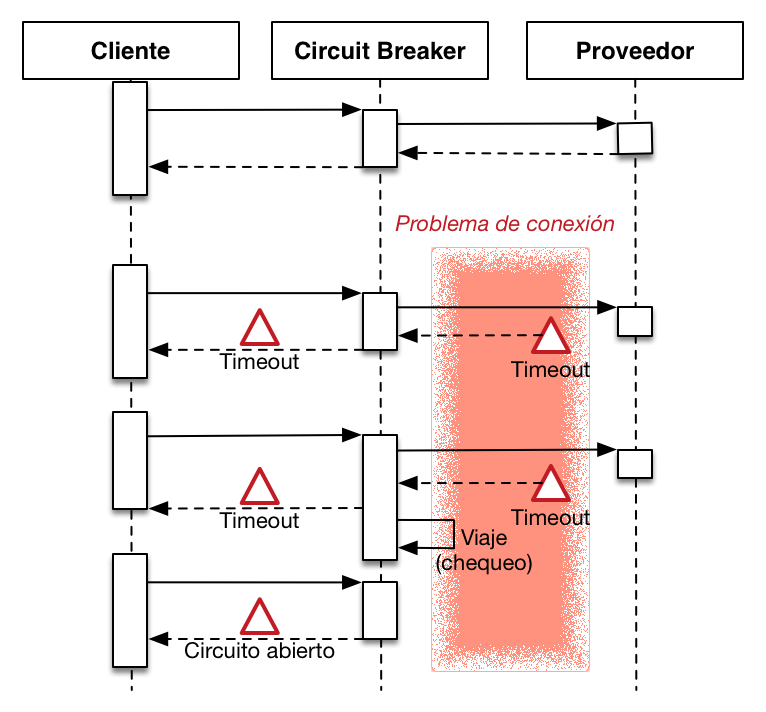
\includegraphics[width=\linewidth,height=0.5\textheight,keepaspectratio]{src/images/04-capitulo-4/circuit-breaker.png}
  \caption{Patrón de tolerancia a fallos \eng{Circuit Breaker}}
  \label{fig:circuit_breaker}
\end{figure}

Para implementar una infraestructura tolerante a fallos, los servicios deberán estar replicados en varias instancias virtuales y, como detallamos anteriomente, delante de éstas se implementará un balanceador de carga que permitirá distribuir las peticiones recibidas entre las instancias virtuales.  Al mismo tiempo, se deberá trabajar en limitar el alcance del fallo a nivel de servicio.  Cabe aclarar que el partón de microservicios, realiza un aporte importante en este orden, ya que al dividir la aplicación en \eng{service components} aislamos el problema, facilitando luego su eventual solución y despliegues en producción.

\subsubsection{Estandarización}

Según el diccionario de la Real Academia Española, un estándar es lo que sirve como tipo, modelo, norma, patrón o referencia. En nuestro caso, la estandarización es el proceso por el cual se establecen normas comúnmente aceptadas que permiten la comunicación de diferentes aplicaciones.

Como mencionamos anteriormente, para cada aplicación que lo requiera se deberá implementar una \gls{acro:api} de acceso a los datos que ésta genere. Esta implementación se realizará basándose en la especificación \nameref{soa:tecnologias:json-api} detallada en la \autoref{soa:tecnologias:para-estructura}.

Esta estandarización facilitará el desarrollo de clientes que consuman información de los diferentes servicios de las \glspl{acro:api}, ya que definen reglas que especifican cómo se podrá acceder a los datos, cuál será su estructura de respuesta, e incluso asisten en lograr independencia del lenguaje con el que se escriban estos clientes, quienes simplemente deben respetar las especificaciones para implementar el acceso a los servicios.

En la \autoref{fig:arquitectura-propuesta} se puede observar la arquitectura final propuesta.

\begin{figure}
  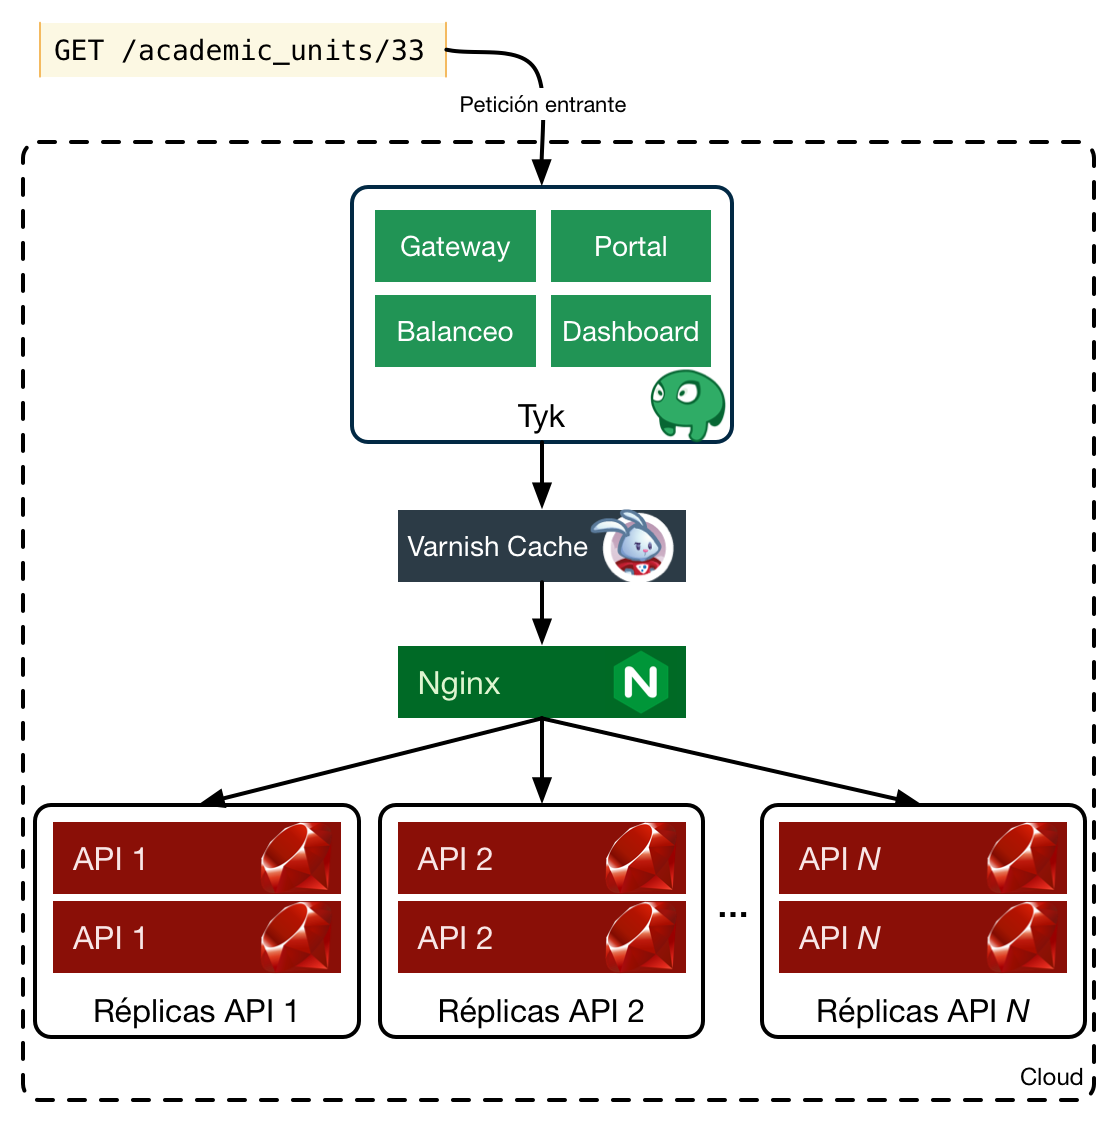
\includegraphics[width=\linewidth]{src/images/04-capitulo-4/propuesta-arquitectura-final.png}
  \caption{Arquitectura propuesta para la {\cloud} de la UNLP}
  \label{fig:arquitectura-propuesta}
\end{figure}
